% ============ CHAPTER 7 — DASHBOARDS ============
\chapter{Dashboards}\label{cha:dashboards}

\section{The web operations dashboard}

The dashboard (\texttt{web/src/App.tsx}, React 18 + TypeScript, served on
port 5173) is the operator- and admin-facing surface. It talks to the
backend over two channels: authenticated REST for every control, and the
backend event stream over WebSocket for live truth. It performs no
transformation of state: what it shows is what the backend published.

\subsection{Login and role awareness}

\begin{itemize}
  \item Login screen posts \texttt{username}/\texttt{password} to
        \texttt{/api/login} (bcrypt-verified) and holds the returned JWT
        in memory for every subsequent REST call.
  \item Three seed roles: \textbf{viewer} observes, \textbf{operator} may
        issue controls, \textbf{admin} additionally inspects the audit
        trail; the UI derives affordances from the role map returned with
        the token, and --- critically --- the backend re-checks every
        request independently, so the UI cannot grant what the token
        forbids.
  \item The top bar shows the authenticated user, the MQTT connection
        state pill (live \texttt{state.mqttConnected}) and a clock.
\end{itemize}

\subsection{Panels and data flow}

Panels\footnote{Panel names are the literal \texttt{<h3>} strings in
\texttt{App.tsx}, observed in the source at the time of writing.} in
rendered order:

\begin{longtable}{>{\raggedright}p{4.6cm} >{\raggedright\arraybackslash}p{5.6cm} >{\raggedright\arraybackslash}p{4.7cm}}
\caption{Dashboard panels}\label{tab:dashpanels}\\
\toprule
\textbf{Panel} & \textbf{Content} & \textbf{Backing data} \\
\midrule
\endfirsthead
\caption[]{(continued)}\\
\toprule
\textbf{Panel} & \textbf{Content} & \textbf{Backing data} \\
\midrule
\endhead
Hero scenario express actions & One-click \texttt{Inject wildlife event} and \texttt{Simulate sensor fault}; an animated scene card with train, live signal head and \texttt{WILDLIFE ZONE} marker & \texttt{POST /api/control} envelope \\
Fleet grid (train cards) & One card per train (T1/T3): current vs target speed, occupied block, UP/DOWN line pill, \texttt{CLOCKWISE}/\texttt{ANTICLOCKWISE} direction; select a card to drive its speed control & retained \texttt{railway/state} snapshot via WS \\
Fleet Speed \& Hazard Controls & Per-train target speed with slider and \texttt{RESET}/\texttt{Clear wildlife}/\texttt{Restore sensor} actions & \texttt{POST /api/speed \{trainId\}}; control envelopes \\
Station Hold Scheduler (meet card) & Meet seed, phase, holder train, chosen route and countdown to next window & \texttt{POST /api/meet}, snapshot \texttt{meets} \\
Wrong-Line Run panel & Operator-requested wrong-line: eligibility display, start and cancel, with hold and clearance states streaming in & \texttt{POST /api/wrong-line}, snapshot \texttt{wrongLine} \\
Sensor $\rightarrow$ Camera $\rightarrow$ Stop (wildlife card) & Stage (\texttt{NONE}/\texttt{SUSPECTED}/\texttt{CONFIRMED}), evidence sources (HUT/CAM/ESP32 tags), confidence, species, camera health (\texttt{ONLINE}/\texttt{DEGRADED}), ML status (\texttt{STUB}/\texttt{LOADED}), near-warning (30\,km/h) & hazard snapshot + \texttt{/api/camera/health} \\
Authoritative Block Signalling \& Occupancy & Block-by-block diagram with per-block aspects (RED/YELLOW/GREEN), occupancy side, CAM/HUT evidence badges on hazard blocks & snapshot blocks + retained \texttt{railway/signal/\{block\}} \\
Audit \& Operations Log & Live event stream (type, message, time, source, severity) --- admin-invisible events are still validated backend-side; audit rows themselves are admin/backend-inspectable & WS event stream \\
Wokwi ESP32 (communicator kernel) & ESP32 device health, zone, telemetry freshness --- the state of the edge node at a glance & \texttt{railway/telemetry/esp32} relay via snapshot \\
\bottomrule
\end{longtable}

\subsection{Evidence badges on the block diagram}

During a hazard, the block diagram tags the involved block with its
evidence sources --- \texttt{CAM} (onboard simulated camera),
\texttt{HUT} (trackside sensor network) or \texttt{ESP32} (edge device) ---
so an operator can immediately see which surfaces agreed, matching the
backend's dual-evidence fusion model (Section~\ref{sec:features-wildlife}).

\section{The twin-side HUD}

The 3D twin carries its own HUD so the information survives even when the
web dashboard is closed:

\begin{itemize}
  \item \textbf{Debug/state bar} (top of every render): zone state,
        signal aspect, \texttt{WILDLIFE}/\texttt{CAM}/\texttt{clear}
        evidence and confidence, sensor health, MQTT connection flag,
        camera status and per-train speed (target and limit) shown in
        \texttt{km/h}.
  \item \textbf{Fleet HUD} (\texttt{test\_fleet\_hud}): per-train lines ---
        speed, block, line, direction --- for both trains simultaneously.
  \item \textbf{Meet HUD} (\texttt{test\_meet\_hud}): phase, holder,
        route and the countdown to the next meet window; tolerated as
        absent when the backend snapshot predates meets.
  \item \textbf{Wrong-line HUD} (\texttt{test\_wrong\_line\_hud}):
        \texttt{WRONG-LINE T1 <phase> <pct>\% T3 HOLD} rendered from the
        backend route state.
  \item \textbf{Camera confirmation HUD}: \texttt{CAM detect}/
        \texttt{CAM clear} plus the confirmed species and confidence ---
        shown in Figure~\ref{fig:cameraconfirm}.
\end{itemize}

\begin{figure}[H]
\centering
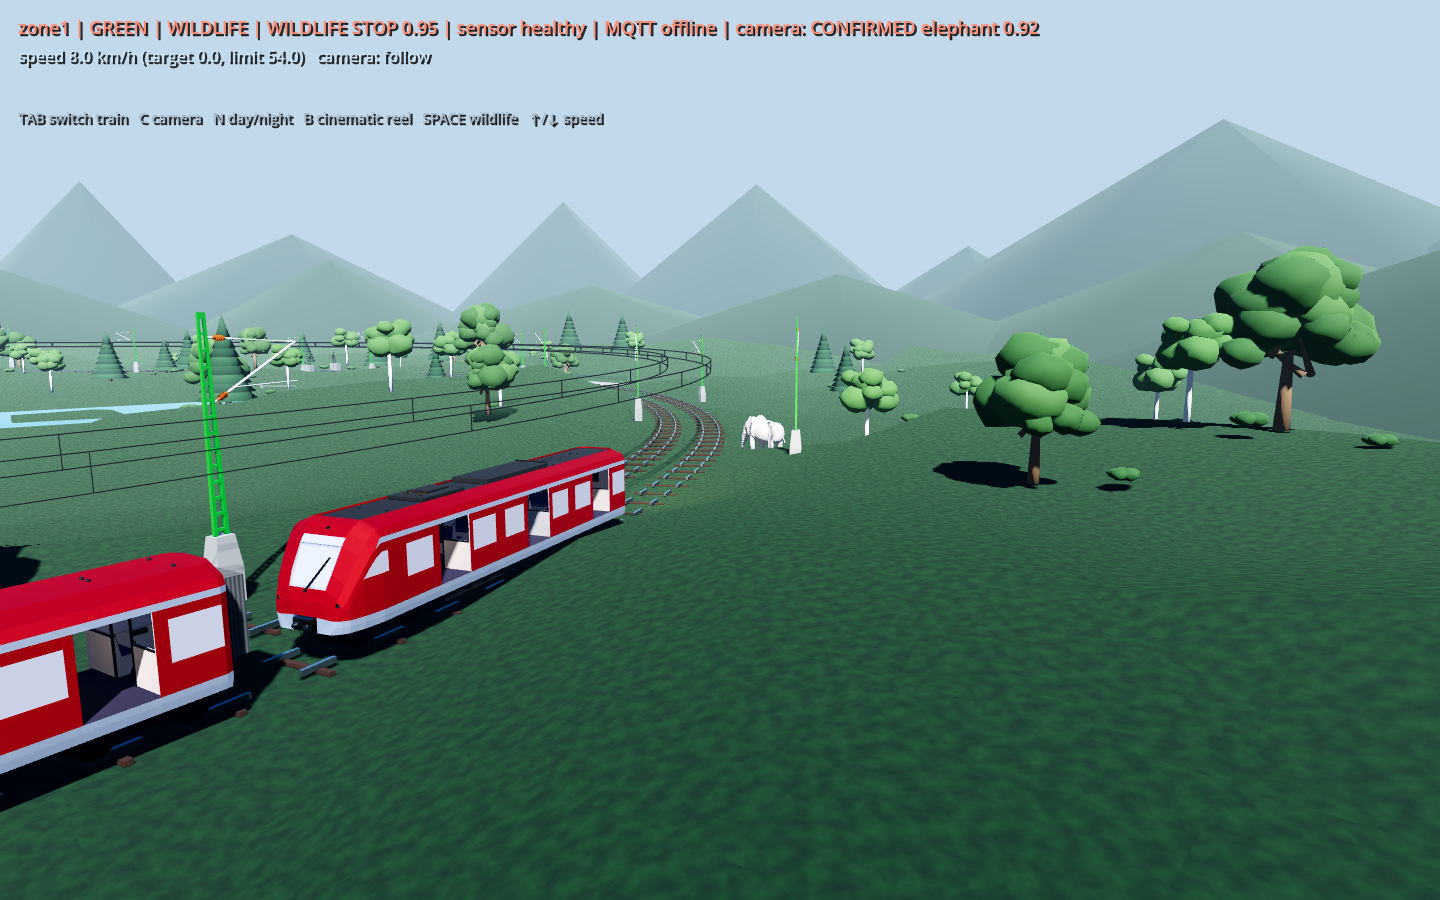
\includegraphics[width=16.8cm]{camera_confirm.png}
\caption{Twin HUD during a confirmed wildlife stop: top bar reads
\texttt{WILDLIFE | WILDLIFE STOP 0.95 | camera: CONFIRMED elephant 0.92}
--- target speed 0, limit 54, camera tracking from behind
the red LTS train. The elephant detection ahead is the simulated render
that produced the confirmed evidence. Captured from
\texttt{capture\_camera\_confirm.gd}.}
\label{fig:cameraconfirm}
\end{figure}

\section{Diagnostics surfaces}

\begin{itemize}
  \item \textbf{Backend health:} \texttt{GET /api/health} returns
        \texttt{\{"ok":true,"mqttConnected":true\}} --- the single command
        every operator first runs (\texttt{dev-up.sh} waits on it for
        up to 60\,s).
  \item \textbf{Audit inspection:} admin surfaces audit rows (actor, role,
        zone, action, result, timestamp) from the SQLite audit table via
        the authenticated endpoint; every control attempt appears here
        regardless of acceptance.
  \item \textbf{Broker observability:} Mosquitto logs all connections;
        ACL denials are visible in \texttt{docker compose logs mqtt} ---
        the fastest way to diagnose a mis-scoped client.
  \item \textbf{Wokwi panel:} the dashboard's ESP32 card exposes the last
        telemetry timestamps, so the edge node's freshness is visible
        without reading serial.
\end{itemize}

\section{Two dashboards, one truth}

A deliberate design property: the web dashboard and the twin HUD are two
renderings of the same backend-published state, and the backend is the
sole publisher. The twin never silently widens permissions, and the
dashboard never invents state: if the twin disagrees with a command, the
discrepancy appears in the HUD's own limit versus the backend's target
(e.g.\ the local limit only \emph{tightens} a target, never loosens it).
